\documentclass[12pt,a4paper,openright]{article}
\usepackage[utf8]{inputenc}
\usepackage[spanish]{babel}
\usepackage{amsmath}
\usepackage{amsfonts}
\usepackage{amssymb}
\usepackage{subfigure}
\usepackage{enumerate}
\usepackage{graphicx}
\usepackage[left=2cm,right=2cm,top=2cm,bottom=2cm]{geometry}
\author{Francisco Javier Real Santoscoy}
\title{Actividad 5}

\begin{document}
\maketitle

\section*{Introducción}

Funciones y subrutinas son subprogramas de FORTRAN. La mayor parte de los problemas son tan complejos que resulta conveniente trocearlos en pequeños problemas que se resuelven en cada función o subrutina.

Generalmente, por cada nivel del diseño descendente se desarrollo un pseudocódigo de alto nivel que hace
uso de acciones no primitivas; si se detecta que alguna de estas acciones no primitivas aparece más de una vez es
posible nombrarla y utilizarla de forma repetida. Tales acciones con nombre se denominan subprogramas y pueden ser,
a su vez, funciones y subrutinas \\

La utilización de subprogramas proporciona múltiples ventajas:
\begin{itemize}
\item Facilitan la modularidad y estructuración de los algoritmos.
\item Facilitan la lectura e inteligibilidad de los algoritmos.
\item Permiten una economización del esfuerzo del programador al poder escribir código reutilizable en muchas
partes de un mismo algoritmo.
\item Facilitan la depuración y mantenimiento de los programas.
\end{itemize}


\subsection*{Funciones}

Una función toma un conjunto de valores como argumentos, realiza algún cálculo y devuelve un único resultado. Hay algunas funciones ya escritas en FORTRAN y que pueden ser usadas por el programador directamente, son las llamadas funciones intrínsecas. La mayor parte son funciones matemáticas.

Las llamadas a funciones nunca
pueden formar una sentencia aislada ni constituir la parte izquierda de una sentencia de asignación.

\subsection*{Subrutinas}

En muchas ocasiones puede interesarnos desarrollar un subprograma que no se vea afectado por las
limitaciones de las funciones; es decir, puede interesarnos un subprograma que sea capaz de “retornar” varios valores o
ninguno. Para esos casos existen las denominadas subrutinas o procedimientos; las subrutinas son subprogramas que
no devuelven ningún resultado, por tanto no tienen tipo, y en los que es “lícito” emplear los efectos laterales antes
mencionados para permitir al programa principal obtener varios valores “resultantes” de la ejecución del subprograma.
Subrutinas actúan de igual forma que las funciones pero pueden devolver varios resultados a la vez. Una subrutina no puede asignarse a una variable pues en si misma no tiene un valor asociado.
En el programa principal una subrutina se activa con la instrucción CALL que incluye el nombre de la subrutina seguida por una lista de inputs y de outputs.
No es necesario declarar el nombre de las subrutinas en el programa principal.
Las subrutinas comienzan por una linea que incluye la palabra SUBROUTINE, el nombre de la subrutina y los argumentos
Todos los argumentos de la subrutina deben de ser declarados en la misma
Una subrutina acaba con un RETURN y un END.


\section*{Actividades a realizar}


Nos interesa utilzar el concepto de funciones en Fortran, para desarrollar una función "Taylor", a la que le demos un par de valores de una función y nos regrese el valor de la Serie de Taylor para un punto.\\

Escriba una función de Taylor en Fortran, que utilice la primera y segunda derivada, por lo que requiere entonces de conocer los valores de una función en $f(x-h)$, $f(x)$  y $f(x+h)$. \\

Utilizando las aproximaciones de diferenciación numérica para la primera y segunda derivada, calcule el error E(x) como función de x, de aproximar con los primeros 3 términos a una función f(x), para los siguientes casos. \\

\begin{enumerate}

\item f(x) = sin(x), alrededor de a=0.
\item f(x) = cos(x), alrededor de a=0.
\item f(x) = tan(x), alrededor de a=0.
\item f(x) = exp(x), alrededor de a=0.

\end{enumerate}
 
 
 Grafique las funciones error $E(x)= f(x) - Taylor(x,a)$, como función de x para cada uno de los casos. \\
 
\begin{large}
 El codigo fuente del programa utilizado
 \end{large} 
 
\begin{verbatim}

program taylorprogram
  
  IMPLICIT NONE

  INTERFACE
     
     FUNCTION SerieTaylor(f_0,f_1,f_2,h)
       REAL :: SerieTaylor
       REAL, INTENT(IN) :: f_0, f_1, f_2, h
     END FUNCTION SerieTaylor
    END INTERFACE
 
  REAL :: x_0, x_1, x_2, h, suma, F
  INTEGER :: i, npts, icaso  
  write(*,*) "Ingresa el numero correspondiente para el caso deseado caso seno: 1 ,coseno: 2 ,tangente: 3 ,exponencial: 4."
  read(*,*) icaso
  write(*,*) icaso  
  npts=21
    
     write(*,*) "Serie de Taylor del Caso Seleccionado Anteriormente"
     h=0.1
   
     do i=1, npts
        x_0=float(i-1)*h
        x_1=float(i)*h
        x_2=float(i+1)*h
       suma =SerieTaylor(F(x_0,icaso), F(x_1,icaso), F(x_2,icaso), h)
     
       write(*,*) i, suma, F(x_1,icaso), (suma-F(x_1,icaso))               
       open(unit=12, file='Error.dat')
       write(12,*)i, suma-F(x_1,icaso)      
     end do
    close(12)
  
   END PROGRAM taylorprogram   
   
   FUNCTION SerieTaylor(f_0,f_1,f_2,h)
    
     IMPLICIT NONE
     REAL :: SerieTaylor
     REAL, INTENT(IN) :: f_0, f_1, f_2, h
     SerieTaylor=f_1+((f_2-f_0)/(2*h))*h+((f_2-2*f_1+f_0)/(2*h*h))*h*h
    
     END FUNCTION SerieTaylor
    
     FUNCTION F(x,icaso)
      
       IMPLICIT NONE
       REAL :: F
       REAL, INTENT(IN) ::  x
       INTEGER, INTENT(IN) :: icaso
       if (icaso.EQ.1) then
          F=sin(x)
       end if      
  
       if (icaso.EQ.2) then
          F=cos(x)
       end if
       if (icaso.EQ.3) then
          F=tan(x)
       end if
       if (icaso.EQ.4) then
          F=exp(x)
       end if  
     
     END FUNCTION F
     

\end{verbatim} 

Las gráficas obtenidas apartir del Codigo. Las graficas muestran el error obtenido entre la medición y la apŕoximación.\\

\begin{figure}[htb]
\centering
\subfigure[Error seno]{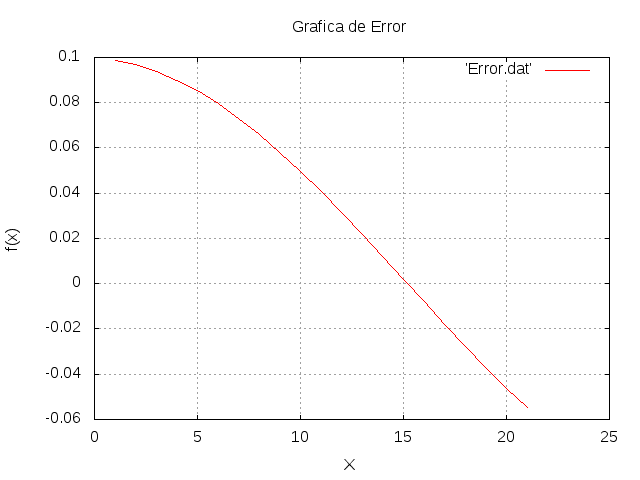
\includegraphics[scale=0.4]{Error1.png}  } \hspace{10mm}
\subfigure[Error Coseno]{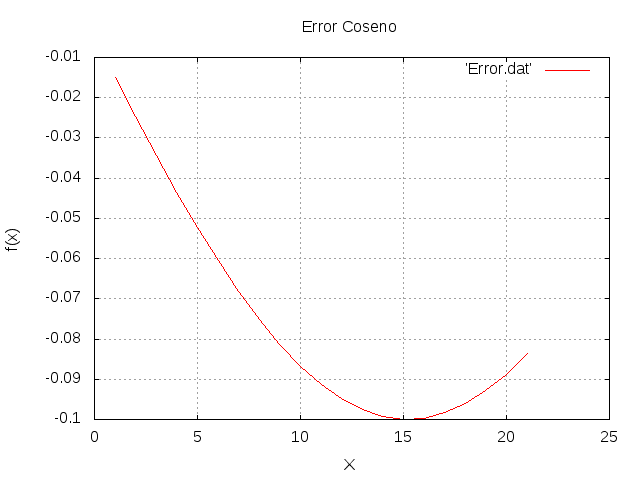
\includegraphics[scale=0.4]{Error2.png}}
\subfigure[Error Tangente]{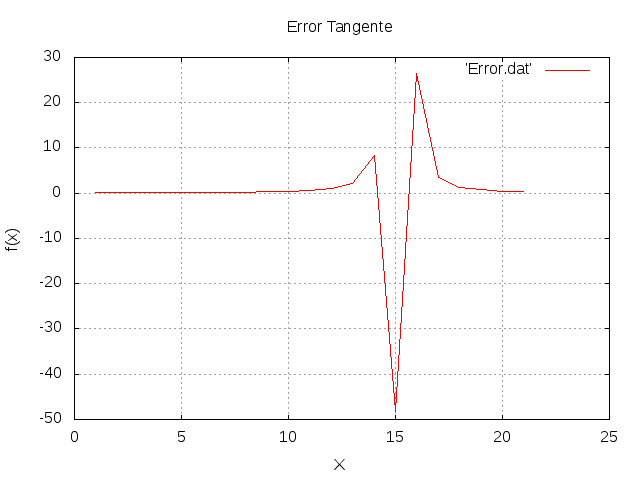
\includegraphics[scale=0.4]{Error3.png}} \hspace{10mm} 
\subfigure[Error Exponencial]{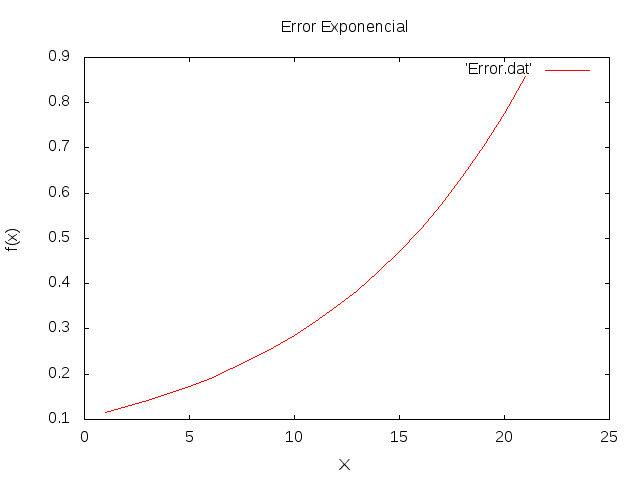
\includegraphics[scale=0.4]{Error4.png}} 
\caption{Errores de las mediciones contra los valores reales} 
\end{figure}




\end{document}